\documentclass[a4paper,12pt]{article}

\usepackage[utf8x]{inputenc}
\usepackage[T2A]{fontenc}
\usepackage[english, russian]{babel}

% Опционно, требует  apt-get install scalable-cyrfonts.*
% и удаления одной строчки в cyrtimes.sty
% Сточку не удалять!
% \usepackage{cyrtimes}

% Картнки и tikz
\usepackage{graphicx}
\usepackage{tikz}
\usetikzlibrary{snakes,arrows,shapes}


% Некоторая русификация.
\usepackage{misccorr}
\usepackage{indentfirst}
\renewcommand{\labelitemi}{\normalfont\bfseries{--}}

% Увы, поля придётся уменьшить из-за листингов.
\topmargin -1cm
\oddsidemargin -0.5cm
\evensidemargin -0.5cm
\textwidth 17cm
\textheight 24cm

\sloppy

% Оглавление в PDF
\usepackage[
bookmarks=true,
colorlinks=true, linkcolor=black, anchorcolor=black, citecolor=black, menucolor=black,filecolor=black, urlcolor=black,
unicode=true
]{hyperref}

% Для исходного кода в тексте
\newcommand{\Code}[1]{\textbf{#1}}

\usepackage{verbatim}
\usepackage{fancyvrb}
\fvset{frame=leftline, fontsize=\small, framerule=0.4mm, rulecolor=\color{darkgray}, commandchars=\\\{\}}
\renewcommand{\theFancyVerbLine}{\small\arabic{FancyVerbLine}}



\title{Отчёт по лабораторной работе \\ <<IP-маршрутизация>>}
\author{Доржсурэн Одсэлмаа}

\begin{document}

\maketitle

\tableofcontents

% Текст отчёта должен быть читаемым!!! Написанное здесь является рыбой.

\section{Топология сети}

Топология сети и использыемые IP-адреса показаны на рис.~\ref{fig:network}.

\begin{figure}
\centering
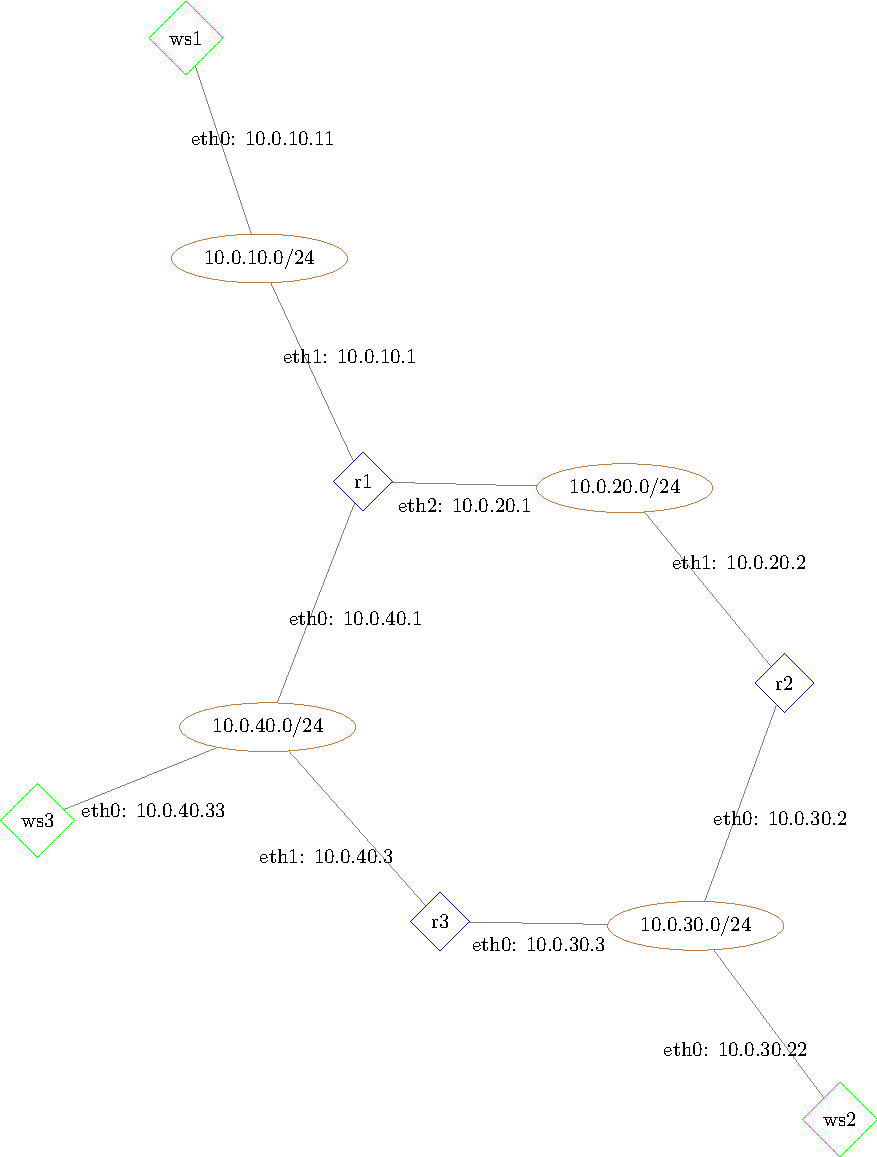
\includegraphics[width=\textwidth]{includes/network_gv.pdf}
\caption{Топология сети}
\label{fig:network}
\end{figure}


\section{Назначение IP-адресов}

Ниже приведён файл настройки протокола IP маршрутизатора \textbf{r1}.


\VerbatimInput{../../net/r1/etc/network/interfaces}

Ниже приведён файл настройки протокола IP рабочей станции \textbf{ws1}.


\VerbatimInput{../../net/ws1/etc/network/interfaces}



\section{Таблица маршрутизации}

Вывести (командой ip r) таблицу маршрутизации для \textbf{r1}.

\begin{Verbatim}
10.0.20.0/24 dev eth2  proto kernel  scope link  src 10.0.20.1 
10.0.30.0/24 via 10.0.20.2 dev eth2 
10.0.40.0/24 dev eth0  proto kernel  scope link  src 10.0.40.1 
10.0.10.0/24 dev eth1  proto kernel  scope link  src 10.0.10.1 
\end{Verbatim}

Вывести (командой ip r) таблицу маршрутизации для \textbf{r2}.

\begin{Verbatim}
10.0.20.0/24 dev eth1  proto kernel  scope link  src 10.0.20.2 
10.0.30.0/24 dev eth0  proto kernel  scope link  src 10.0.30.2 
10.0.40.0/24 via 10.0.30.3 dev eth0 
10.0.10.0/24 via 10.0.20.1 dev eth1 

\end{Verbatim}
Вывести (командой ip r) таблицу маршрутизации для \textbf{r3}.
\begin{Verbatim}
10.0.20.0/24 via 10.0.30.2 dev eth0 
10.0.30.0/24 dev eth0  proto kernel  scope link  src 10.0.30.3 
10.0.40.0/24 dev eth1  proto kernel  scope link  src 10.0.40.3 
10.0.10.0/24 via 10.0.40.1 dev eth1 
\end{Verbatim}

Вывести (командой ip r) таблицу маршрутизации для \textbf{ws1}.
\begin{Verbatim}
10.0.10.0/24 dev eth0  proto kernel  scope link  src 10.0.10.11 
default via 10.0.10.1 dev eth0 
\end{Verbatim}

Вывести (командой ip r) таблицу маршрутизации для \textbf{ws2}.
\begin{Verbatim}
10.0.30.0/24 dev eth0  proto kernel  scope link  src 10.0.30.22 
default via 10.0.30.3 dev eth0 
\end{Verbatim}

Вывести (командой ip r) таблицу маршрутизации для \textbf{ws3}.
\begin{Verbatim}
10.0.40.0/24 dev eth0  proto kernel  scope link  src 10.0.40.33 
default via 10.0.40.1 dev eth0 
\end{Verbatim}



% ... Повторять для всех маршрутизаторов и рабочих станций, где есть что-то кроме gateway.

\section{Проверка настройки сети}

Вывод \textbf{traceroute} от узла \textbf{ws1} до \textbf{ws3} при нормальной работе сети.

\begin{Verbatim}
 1  10.0.10.1  9 ms  0 ms  0 ms
 2  10.0.40.33  11 ms  0 ms  0 ms

\end{Verbatim}

Вывод \textbf{traceroute} от узла \textbf{r1} до \textbf{ws2} при нормальной работе сети.

\begin{Verbatim}
 1  10.0.20.2  2 ms  0 ms  0 ms
 2  10.0.30.22  26 ms  0 ms  0 ms

\end{Verbatim}

Вывод \textbf{traceroute} от узла \textbf{w1} до \textbf{r2} при нормальной работе сети.

\begin{Verbatim}
 1  10.0.10.1  5 ms  0 ms  0 ms
 2  10.0.20.2  0 ms  0 ms  0 ms
\end{Verbatim}


\section{Маршрутизация}

% На пути здесь достаточно быть одному аршрутизатору!

Вначале стоит написать, какие MAC-адреса интерфейсов в опыте были у каких машин.
\begin{Verbatim}
ws1 eth0:  a6:f9:52:b6:1e:69 
r1 eth1: fa:de:dc:30:96:57  
r1 eth2: 46:9d:1d:7c:12:b2 
r2 eth1: 12:3e:e2:7d:e3:87
\end{Verbatim}


Затем вывести маршрутную таблицу маршрутизатора \textbf{r1} (вывод команды ip r!)

\begin{Verbatim}
10.0.20.0/24 dev eth1  proto kernel  scope link  src 10.0.20.2 
10.0.30.0/24 dev eth0  proto kernel  scope link  src 10.0.30.2 
10.0.40.0/24 via 10.0.30.3 dev eth0 
10.0.10.0/24 via 10.0.20.1 dev eth1 
\end{Verbatim}

Показаны опыты после стирания кеша ARP.
% Не забудьте это сделать!
Далее показана отправка пакета на маршрутизатор \textbf{r2} (косвенная маршрутизация). 

\begin{Verbatim}
ws1:~# ping 10.0.30.2 -c 1
\end{Verbatim}

\begin{Verbatim}
r1:~# tcpdump -tne -i eth1
a6:f9:52:b6:1e:69 > ff:ff:ff:ff:ff:ff, ethertype ARP (0x0806), length 42: 
	arp who-has 10.0.10.1 tell 10.0.10.11
fa:de:dc:30:96:57 > a6:f9:52:b6:1e:69, ethertype ARP (0x0806), length 42: 
	arp reply 10.0.10.1 is-at fa:de:dc:30:96:57
a6:f9:52:b6:1e:69 > fa:de:dc:30:96:57, ethertype IPv4 (0x0800), length 98: 
	10.0.10.11 > 10.0.20.2: ICMP echo request, id 12546, seq 1, length 64
fa:de:dc:30:96:57 > a6:f9:52:b6:1e:69, ethertype IPv4 (0x0800), length 98: 
	10.0.20.2 > 10.0.10.11: ICMP echo reply, id 12546, seq 1, length 64
fa:de:dc:30:96:57 > a6:f9:52:b6:1e:69, ethertype ARP (0x0806), length 42: 
	arp who-has 10.0.10.11 tell 10.0.10.1
a6:f9:52:b6:1e:69 > fa:de:dc:30:96:57, ethertype ARP (0x0806), length 42: 
	arp reply 10.0.10.11 is-at a6:f9:52:b6:1e:69
\end{Verbatim}

Затем маршрутизатор отправил его далее.

\begin{Verbatim}
r2:~# tcpdump -tne -i eth1
46:9d:1d:7c:12:b2 > ff:ff:ff:ff:ff:ff, ethertype ARP (0x0806), length 42: 
	arp who-has 10.0.20.2 tell 10.0.20.1
12:3e:e2:7d:e3:87 > 46:9d:1d:7c:12:b2, ethertype ARP (0x0806), length 42: 
	arp reply 10.0.20.2 is-at 12:3e:e2:7d:e3:87
46:9d:1d:7c:12:b2 > 12:3e:e2:7d:e3:87, ethertype IPv4 (0x0800), length 98:
	10.0.10.11 > 10.0.20.2: ICMP echo request, id 12546, seq 1, length 64
12:3e:e2:7d:e3:87 > 46:9d:1d:7c:12:b2, ethertype IPv4 (0x0800), length 98: 
	10.0.20.2 > 10.0.10.11: ICMP echo reply, id 12546, seq 1, length 64
12:3e:e2:7d:e3:87 > 46:9d:1d:7c:12:b2, ethertype ARP (0x0806), length 42: 
	arp who-has 10.0.20.1 tell 10.0.20.2
46:9d:1d:7c:12:b2 > 12:3e:e2:7d:e3:87, ethertype ARP (0x0806), length 42: 
	arp reply 10.0.20.1 is-at 46:9d:1d:7c:12:b2

\end{Verbatim}

\section{Продолжительность жизни пакета}

Сначала написать как и на чём ломали. 

\begin{Verbatim}
r2:~# ip link set eth0 down
r2:~# ip route add 10.0.30.0/24 via 10.0.20.1 dev eth1
\end{Verbatim}

Потом какая-то таблица вышла.

\begin{Verbatim}
r2:~# ip r
10.0.20.0/24 dev eth1  proto kernel  scope link  src 10.0.20.2 
10.0.30.0/24 via 10.0.20.1 dev eth1 
10.0.10.0/24 via 10.0.20.1 dev eth1 
\end{Verbatim}

Потом что слали.

\begin{Verbatim}
ws1:~# ping 10.0.30.22 -c 1
\end{Verbatim}

И что в итоге получилось.

\begin{Verbatim}
r2:~# tcpdump -tnve -i eth1
tcpdump: listening on eth1, link-type EN10MB (Ethernet), capture size 96 bytes
46:9d:1d:7c:12:b2 > 12:3e:e2:7d:e3:87, ethertype IPv4 (0x0800), length 98: 
	(tos 0x0, ttl 63, id 0, offset 0, flags [DF], proto ICMP (1), length 84) 
	10.0.10.11 > 10.0.30.22: ICMP echo request, id 14850, seq 1, length 64
12:3e:e2:7d:e3:87 > 46:9d:1d:7c:12:b2, ethertype IPv4 (0x0800), length 98: 
	(tos 0x0, ttl 62, id 0, offset 0, flags [DF], proto ICMP (1), length 84) 
	10.0.10.11 > 10.0.30.22: ICMP echo request, id 14850, seq 1, length 64
...
12:3e:e2:7d:e3:87 > 46:9d:1d:7c:12:b2, ethertype IPv4 (0x0800), length 98: 
	(tos 0x0, ttl 2, id 0, offset 0, flags [DF], proto ICMP (1), length 84) 
	10.0.10.11 > 10.0.30.22: ICMP echo request, id 14850, seq 1, length 64
46:9d:1d:7c:12:b2 > 12:3e:e2:7d:e3:87, ethertype IPv4 (0x0800), length 98: 
	(tos 0x0, ttl 1, id 0, offset 0, flags [DF], proto ICMP (1), length 84) 
	10.0.10.11 > 10.0.30.22: ICMP echo request, id 14850, seq 1, length 64
12:3e:e2:7d:e3:87 > 46:9d:1d:7c:12:b2, ethertype IPv4 (0x0800), length 126: 
	(tos 0xc0, ttl 64, id 49216, offset 0, flags [none], proto ICMP (1), length 112) 
	10.0.20.2 > 10.0.10.11: ICMP time exceeded in-transit, length 92
	(tos 0x0, ttl 1, id 0, offset 0, flags [DF], proto ICMP (1), length 84) 
	10.0.10.11 > 10.0.30.22: ICMP echo request, id 14850, seq 1, length 64


\end{Verbatim}

И кто в итоге отравил сообщение о завершении жизни.
\begin{Verbatim}
ws1:~# ping 10.0.30.22 -c 1
PING 10.0.30.22 (10.0.30.22) 56(84) bytes of data.
From 10.0.20.2 icmp_seq=1 Time to live exceeded

--- 10.0.30.22 ping statistics ---
1 packets transmitted, 0 received, +1 errors, 100% packet loss, time 0ms
\end{Verbatim}


\section{Изучение IP-фрагментации}

Написать, на каких узлах и как изменяли MTU.


\begin{Verbatim}
r1:~# ip link set dev eth2 mtu 576
\end{Verbatim}

\begin{Verbatim}
r2:~# ip link set dev eth1 mtu 576
\end{Verbatim}

% Напоминаем, что PMTU следует отключить!

Какие команды давали для тестирования и где.

\begin{Verbatim}
ws1:~# ping -c 1 -s 1000 10.0.30.22
\end{Verbatim}

Вывод \textbf{tcpdump} на маршрутизаторе перед сетью с уменьшенным MTU.

% Вывод в ширину можно и сократить, удалив несущественные моменты!

\begin{Verbatim}
r1:~# tcpdump -tnv -i eth1 icmp 
tcpdump: listening on eth1, link-type EN10MB (Ethernet), capture size 96 bytes
IP (tos 0x0, ttl 64, id 18648, offset 0, flags [none], proto ICMP (1), length 1028) 10.0.10.11 > 10.0.30.22: ICMP echo request, id 12034, seq 1, length 1008
IP (tos 0x0, ttl 62, id 18125, offset 0, flags [none], proto ICMP (1), length 1028) 10.0.30.22 > 10.0.10.11: ICMP echo reply, id 12034, seq 1, length 1008
\end{Verbatim}

Вывод \textbf{tcpdump} на маршрутизаторе после сети с уменьшенным MTU.

% Вывод в ширину можно и сократить, удалив несущественные моменты!

\begin{Verbatim}
r2:~# tcpdump -tnv -i eth1 icmp
tcpdump: listening on eth1, link-type EN10MB (Ethernet), capture size 96 bytes
IP (tos 0x0, ttl 63, id 18648, offset 0, flags [+], proto ICMP (1), length 572) 10.0.10.11 > 10.0.30.22: ICMP echo request, id 12034, seq 1, length 552
IP (tos 0x0, ttl 63, id 18648, offset 552, flags [none], proto ICMP (1), length 476) 10.0.10.11 > 10.0.30.22: icmp
\end{Verbatim}


Вывод \textbf{tcpdump} на узле получателя.

\begin{Verbatim}
ws2:~# tcpdump -tnv -i eth0 icmp
tcpdump: listening on eth0, link-type EN10MB (Ethernet), capture size 96 bytes
IP (tos 0x0, ttl 62, id 18648, offset 0, flags [none], proto ICMP (1), length 1028) 10.0.10.11 > 10.0.30.22: ICMP echo request, id 12034, seq 1, length 1008
IP (tos 0x0, ttl 64, id 18125, offset 0, flags [none], proto ICMP (1), length 1028) 10.0.30.22 > 10.0.10.11: ICMP echo reply, id 12034, seq 1, length 1008
\end{Verbatim}


\section{Отсутствие сети}

Аналогично опишите опыт, когда маршрутизатор отсылает сообщение об отсутствии с сети.
С командами и выводом, мак адреса не нужны.
\begin{Verbatim}
ws1:~# ping -c 1 10.1.30.22
PING 10.1.30.22 (10.1.30.22) 56(84) bytes of data.
From 10.0.10.1 icmp_seq=1 Destination Net Unreachable
\end{Verbatim}
\begin{Verbatim}
r1:~# tcpdump -n -i eth1 icmp 
13:25:22.808880 IP 10.0.10.11 > 10.1.30.22: ICMP echo request, id 13058, seq 1, length 64
13:25:22.808897 IP 10.0.10.1 > 10.0.10.11: ICMP net 10.1.30.22 unreachable, length 92
\end{Verbatim}
\section{Отсутствие IP-адреса в сети}

Аналогично опишите опыт, когда маршрутизатор отсылает сообщение об отстутствии требуемого IP-адреса в сети.
С командами и выводом, мак адреса не нужны.
\begin{Verbatim}
ws1:~# ping -c 1 10.0.20.254
PING 10.0.20.254 (10.0.20.254) 56(84) bytes of data.
From 10.0.10.1 icmp_seq=1 Destination Host Unreachables
\end{Verbatim}
\begin{Verbatim}
r1:~# tcpdump -n -i eth1 
tcpdump: verbose output suppressed, use -v or -vv for full protocol decode
listening on eth1, link-type EN10MB (Ethernet), capture size 96 bytes
13:32:13.144890 IP 10.0.10.11 > 10.0.20.254: ICMP echo request, id 14594, seq 1, length 64
13:32:16.149622 IP 10.0.10.1 > 10.0.10.11: ICMP host 10.0.20.254 unreachable, length 92
13:32:18.142925 arp who-has 10.0.10.1 tell 10.0.10.11
13:32:18.142939 arp reply 10.0.10.1 is-at fa:de:dc:30:96:57
\end{Verbatim}

\end{document}
